\section{Lecture 12: Online PCA and Hebbian Learning}

The second lecture starts from the PCA eigenproblem and asks a more biological and algorithmic question: can the leading principal directions be learned incrementally, without first forming and diagonalizing the full covariance matrix?

The answer is yes. A linear neuron with a simple Hebbian update performs a stochastic version of the power method. With normalization, the update becomes Oja's rule and converges to the first principal component. With multiple neurons and orthogonalization, Sanger's generalized Hebbian algorithm extracts several principal components. With the sign reversed, anti-Hebbian learning can instead find small-variance directions, which act as novelty filters.

\subsection{PCA As A Learning Problem}

For centered observations \(x^{(\alpha)}\in\mathbb{R}^N\), the covariance matrix is
\[
  C
  =
  \frac{1}{p}
  \sum_{\alpha=1}^{p}
  x^{(\alpha)}x^{(\alpha)\mathsf{T}}.
\]
PCA asks for the unit vector \(e\) that maximizes projected variance:
\[
  e_1
  =
  \operatorname*{arg\,max}_{\|e\|=1}
  e^{\mathsf{T}}Ce.
\]
The stationary condition is the eigenvalue equation
\[
  Ce=\lambda e.
\]
So the first principal component is the eigenvector with the largest eigenvalue.

The offline solution computes \(C\) and diagonalizes it. Online PCA instead sees one pattern at a time and updates a weight vector. The data stream is turned into a dynamical system whose stable direction is the first principal component.

\subsection{A Linear Neuron}

The model neuron in the lecture is deliberately simple:
\[
  y=w^{\mathsf{T}}x.
\]
The input \(x\) is a centered observation, \(w\) is the synaptic weight vector, and \(y\) is the scalar output. The output is large when the input aligns with the current weight vector.

This model is useful because the same expression appears in PCA. The projection of \(x\) onto a candidate direction \(w\) is exactly \(w^{\mathsf{T}}x\). Learning \(w\) is therefore learning a projection direction.

\subsection{Hebb's Rule Finds The Dominant Direction}

Hebbian learning is summarized by the phrase: units that are active together should strengthen their connection. For the linear neuron, the update is
\[
  \Delta w
  =
  \varepsilon yx,
\]
or componentwise,
\[
  \Delta w_j
  =
  \varepsilon yx_j.
\]
The learning rate \(\varepsilon>0\) is small. Each sample nudges the weights in the direction of the current input, scaled by the output. Inputs that already align with \(w\) produce larger outputs and therefore larger changes.

To see why this is PCA, average the update over many centered samples:
\[
  \mathbb{E}[\Delta w]
  =
  \varepsilon \mathbb{E}[yx]
  =
  \varepsilon \mathbb{E}[xx^{\mathsf{T}}]w
  =
  \varepsilon Cw.
\]
The mean update is multiplication by the covariance matrix. This is the same operation used by the power method.

Let \(e_1,\dots,e_N\) be the eigenvectors of \(C\), with eigenvalues
\[
  \lambda_1>\lambda_2>\cdots>\lambda_N.
\]
Write the weight vector in this eigenbasis:
\[
  w=a_1e_1+a_2e_2+\cdots+a_Ne_N.
\]
Since \(Ce_j=\lambda_j e_j\), the averaged update gives
\[
  \Delta a_j
  =
  \varepsilon \lambda_j a_j.
\]
The coefficient along \(e_1\) grows fastest because \(\lambda_1\) is largest. If the initial weight vector has any nonzero component in the \(e_1\) direction, the direction of \(w\) approaches \(e_1\).

The problem is the norm. Pure Hebbian learning does not keep \(\|w\|\) fixed. The direction becomes useful, but the weight length diverges.

\subsection{Oja's Rule Adds The Missing Constraint}

PCA is a constrained optimization problem: the direction \(e\) must have unit norm. Oja's rule builds that constraint into the learning rule:
\[
  \Delta w
  =
  \varepsilon y(x-yw).
\]
In components,
\[
  \Delta w_j
  =
  \varepsilon y(x_j-yw_j).
\]
The first term, \(\varepsilon yx\), is the Hebbian attraction term. The second term, \(-\varepsilon y^2w\), is a stabilizing decay term that grows when the output is large. It prevents the weight vector from increasing without bound.

One way to understand Oja's rule is explicit normalization. Start with a Hebbian step,
\[
  \tilde{w}=w+\varepsilon yx,
\]
then normalize,
\[
  w_{\mathrm{new}}
  =
  \frac{\tilde{w}}{\|\tilde{w}\|}.
\]
For small \(\varepsilon\), a Taylor expansion gives the Oja update to first order:
\[
  w_{\mathrm{new}}-w
  \approx
  \varepsilon y(x-yw).
\]
So Oja's rule is a local, online approximation to Hebbian learning plus Euclidean normalization.

\begin{figure}[h]
\centering
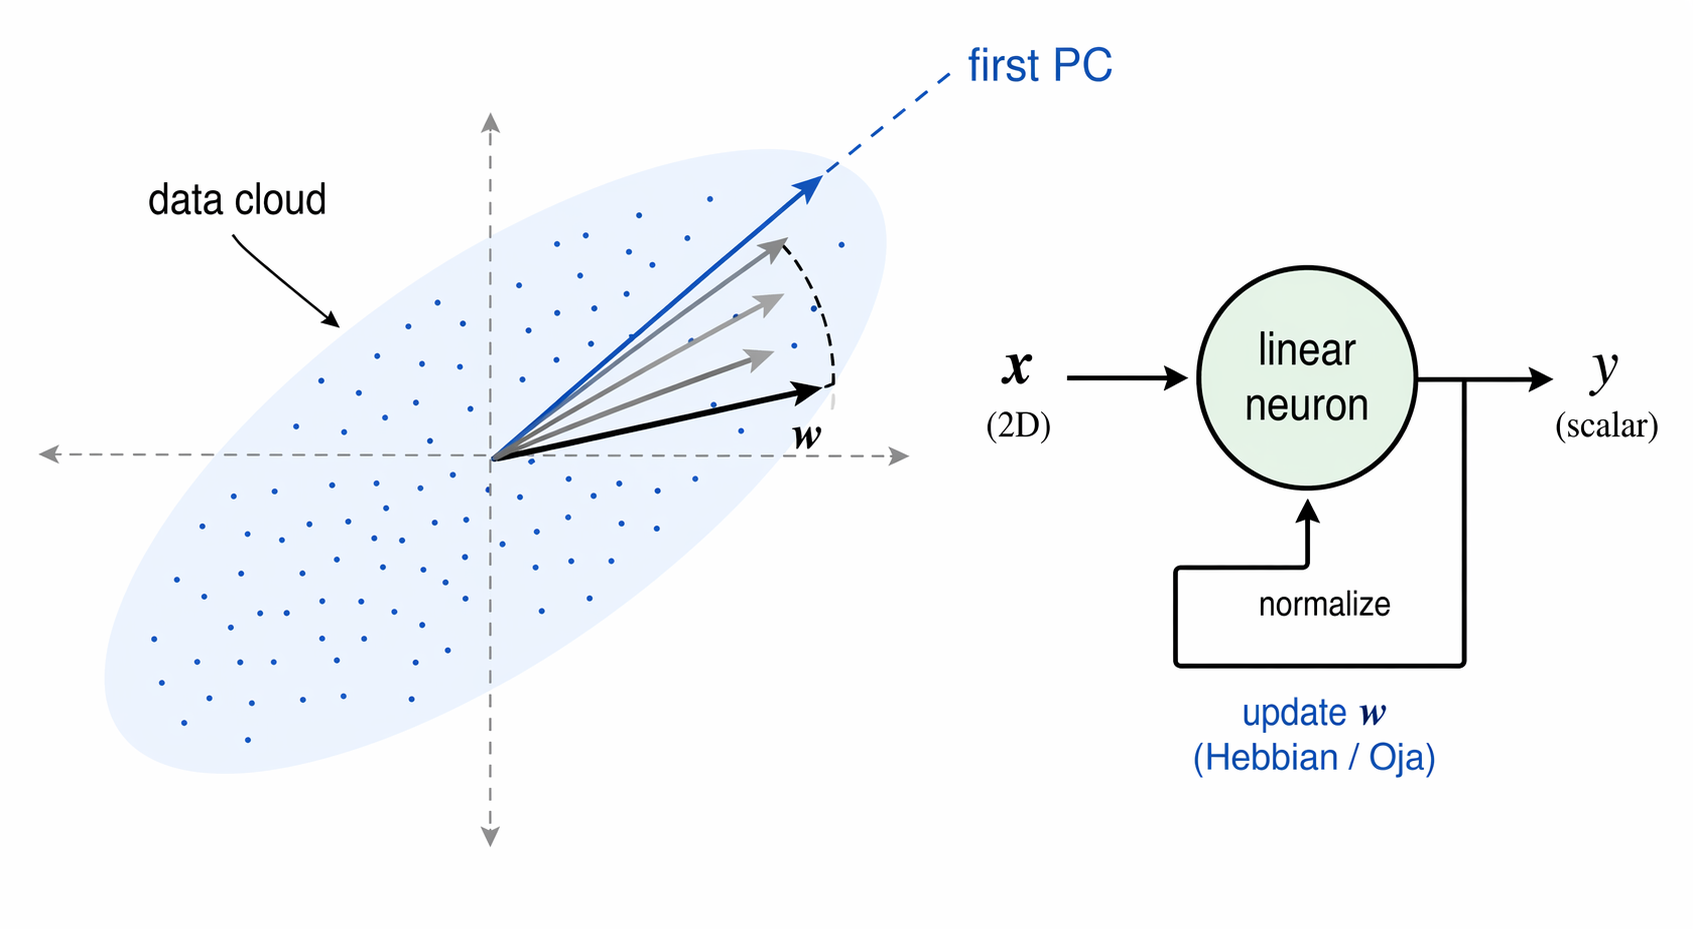
\includegraphics[width=0.96\textwidth]{figures/hebbian/online-pca-oja.png}
\caption{Online PCA with one linear neuron. Hebbian updates rotate the weight vector toward the high-variance direction of the centered data cloud. Oja's normalization keeps the vector length bounded, so the stable direction is the first principal component.}
\end{figure}

\subsection{The Fixed Point Intuition}

At convergence under Oja's rule, \(w\) is a unit vector aligned with the leading eigenvector. The averaged update is zero when the Hebbian growth is exactly balanced by the normalization term. If \(w=e_1\), then
\[
  \mathbb{E}[yx]
  =
  Cw
  =
  \lambda_1 w,
\]
and
\[
  \mathbb{E}[y^2]
  =
  w^{\mathsf{T}}Cw
  =
  \lambda_1.
\]
Thus the mean update becomes
\[
  \varepsilon(Cw-\mathbb{E}[y^2]w)
  =
  \varepsilon(\lambda_1w-\lambda_1w)
  =
  0.
\]
The leading eigenvector is stable because any small component along a lower-variance direction grows more slowly than the leading component.

\subsection{From One Component To Many: Sanger's Rule}

One neuron learns one principal direction. To learn several directions, the system needs multiple neurons and a mechanism that prevents them all from converging to the same first component.

Let
\[
  y_i=w_i^{\mathsf{T}}x
\]
be the output of neuron \(i\). Sanger's generalized Hebbian algorithm uses
\[
  \Delta w_i
  =
  \varepsilon y_i
  \left(
    x-\sum_{k=1}^{i}y_kw_k
  \right).
\]
Componentwise this is
\[
  \Delta w_{ij}
  =
  \varepsilon y_i
  \left(
    x_j-\sum_{k=1}^{i}w_{kj}y_k
  \right).
\]
For \(i=1\), this is Oja's rule. For \(i=2\), the input is first stripped of the component already explained by \(w_1\). For \(i=3\), the input is stripped of the components explained by \(w_1\) and \(w_2\), and so on.

The rule is therefore an online Gram-Schmidt procedure. Each neuron performs Oja-like learning on the residual left after earlier neurons have taken their directions. Under the usual assumptions, the weights converge to the ordered principal components:
\[
  w_1\to e_1,\qquad
  w_2\to e_2,\qquad
  \dots,\qquad
  w_M\to e_M.
\]
After learning, the neuron outputs are the PCA scores:
\[
  y_i=e_i^{\mathsf{T}}x.
\]

\begin{figure}[h]
\centering
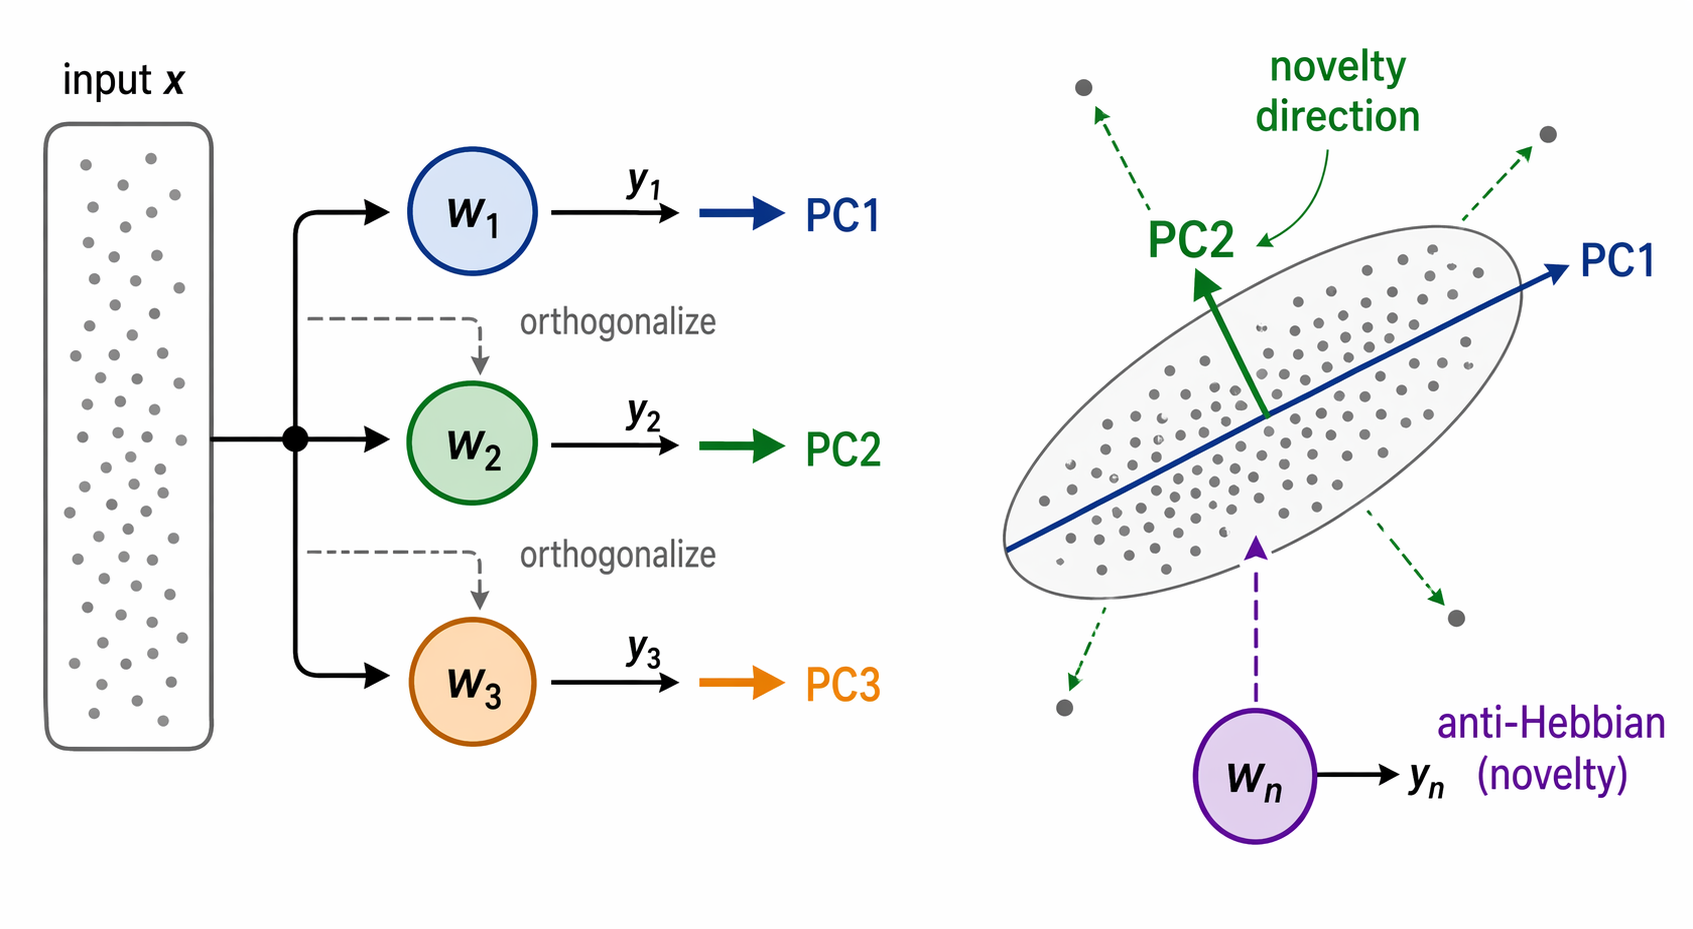
\includegraphics[width=0.96\textwidth]{figures/hebbian/sanger-novelty.png}
\caption{Multiple Hebbian neurons need competition or orthogonalization. Sanger's rule makes each later neuron learn from the residual left by earlier neurons, producing ordered principal components. Reversing the sign gives an anti-Hebbian novelty direction aligned with low-variance structure.}
\end{figure}

\subsection{Novelty Filters And Anti-Hebbian Learning}

Large-variance directions describe what is common. Small-variance directions can reveal what is surprising. If the data normally lie near a low-dimensional manifold, then a point with a large projection onto a small-variance direction is unusual.

The lecture expresses this with the last principal component. After PCA learning,
\[
  y=e_N^{\mathsf{T}}x
\]
is the projection onto the direction with the smallest eigenvalue. A large absolute value of \(y\) signals that the input has energy in a direction where normal data vary little. This is the novelty-filter idea.

The online rule is anti-Hebbian:
\[
  \Delta w
  =
  -\varepsilon yx.
\]
Averaging gives
\[
  \mathbb{E}[\Delta w]
  =
  -\varepsilon Cw.
\]
In the eigenbasis,
\[
  \Delta a_j
  =
  -\varepsilon \lambda_j a_j.
\]
Large-eigenvalue components decay fastest. With normalization, the remaining direction is the eigenvector with the smallest eigenvalue. A normalized anti-Hebbian version of Oja's rule therefore converges to \(e_N\).

\subsection{Connection To Total Least Squares}

The novelty-filter direction also appears in linear regression geometry. Ordinary least squares minimizes vertical residuals and is correct when noise is only in the dependent variable. If both coordinates are noisy, a more symmetric objective is total least squares: minimize orthogonal distances to a line.

For centered two-dimensional data, the normal vector \(w\) to the best-fit line solves
\[
  \min_{\|w\|=1}
  w^{\mathsf{T}}Cw.
\]
This is the opposite of the first PCA objective. Maximizing \(w^{\mathsf{T}}Cw\) gives the high-variance direction along the data. Minimizing it gives the low-variance normal direction. The solution is the normalized eigenvector of \(C\) with the smallest eigenvalue.

\subsection{Summary}

Hebbian learning turns PCA from an offline spectral computation into an online dynamical process. Pure Hebbian learning performs covariance multiplication and therefore points toward the first principal component, but its norm diverges. Oja's rule adds normalization and stabilizes the first component. Sanger's rule adds sequential orthogonalization so multiple neurons learn ordered principal components. Anti-Hebbian learning reverses the direction of the dynamics and, with normalization, finds low-variance novelty directions.
